\chapter{Introduction}\label{introduction}

Bird flocking is a natural phenomenon which always appears in group activities like collective hunting, entertainment or migration. Biologists have found that the flocking behavior benefits the entire colony by improving the overall foraging~\cite{Foraging}, predators spotting~\cite{Predator} and propagation~\cite{Propagation} efficiency. Specifically, the allocation of individual tasks, communication and motion control of each agent has determined the main characteristics of the flock system, such as the scalability, robustness and convergence rate. Studies regarding the motion control and the realization of bird flocking with mobile robots, with no doubt, will greatly inspire the human beings.

There are three important criteria to describe a stable flocking system: separation, cohesion and alignment~\cite{Reynolds1987}. Alignment criterion requires each agent to match self's velocity with neighboring flockmates in the mid range, separation criterion requires each agent to repel neighboring flockmates in the short range and cohesion criterion requires each agent to steer neighboring flockmates in the long range. The faster a flock converges from division and the quicker $\psi_{scal}$ (\ref{eq:psi_scal}) gets close to 1, the more robust the system is. $N$ is the number of total agents, $v_i$ is a vector denoting the velocity of $i^{th}$ agent in the flock.

\begin{equation}\label{eq:psi_scal}
\psi_{scal}(t)=\frac{1}{N(N-1)}\sum^N_{i=1}\sum_{j\neq i}\frac{v_i(t)v_j(t)}{|v_i(t)||v_j(t)|}
\end{equation}

To study the individual agents and realize the flocking system, quadrotors or unmanned aerial vehicles (UAVs) are selected owing to their flexibility and mobility in 3D space. Today, the capability of a single UAV has been increasing rapidly, accompanied by the falling prices and improving performance of the communication, sensing and processing hardwares. Meanwhile, the measurement and control of the UAVs in flock realization are expected to be distributed. Realization with distributed measurement requires all the information to be collected by sensors on-board, such as LiDAR, inertial measurement unit (IMU) or camera instead of external positioning systems like GPS~\cite{Vicsek2018}, motion capture system~\cite{Swarm2018,MPC} or real-time kinematic system (RTK). Realization with distributed control requires each UAV to decide its movement with information available at that agent~\cite{MAV2017} instead of executing commands from a central computer~\cite{CAPT,POMDP,Kumar2018} or a leader UAV. The assumption of distributed architecture agrees with the nature that individual agents react to their sensed environment and surrounding neighbors.

There are mainly two methods to achieve UAV flockings at present, virtual structure and behavior-based methods. Virtual structure method treats the entire UAVs as a virtual single rigid body where the relative pose between each UAV and the virtual geometry center is kept~\cite{Virtual2008,Askari2015,Cai2012,RAS,Distributed,LQR2014,VirtualLeader,Bearing2016}, however, internal communication is sometimes inevitable and altering flocking shape is inflexible when facing dynamically changing environment. In behavior-based approach, control functions are separated into variety of function items and the whole function is then formed as the combination of different items~\cite{Zhang2018,Martin2014,Vicsek2018,VLAP,Behavior2004}, however, this method suffers from undesirable local minima and the convergence of the flocking is not promising.

\begin{figure}[htb]
  \centering
  \subfigure[Indoor environment.]{\label{fig:indoor}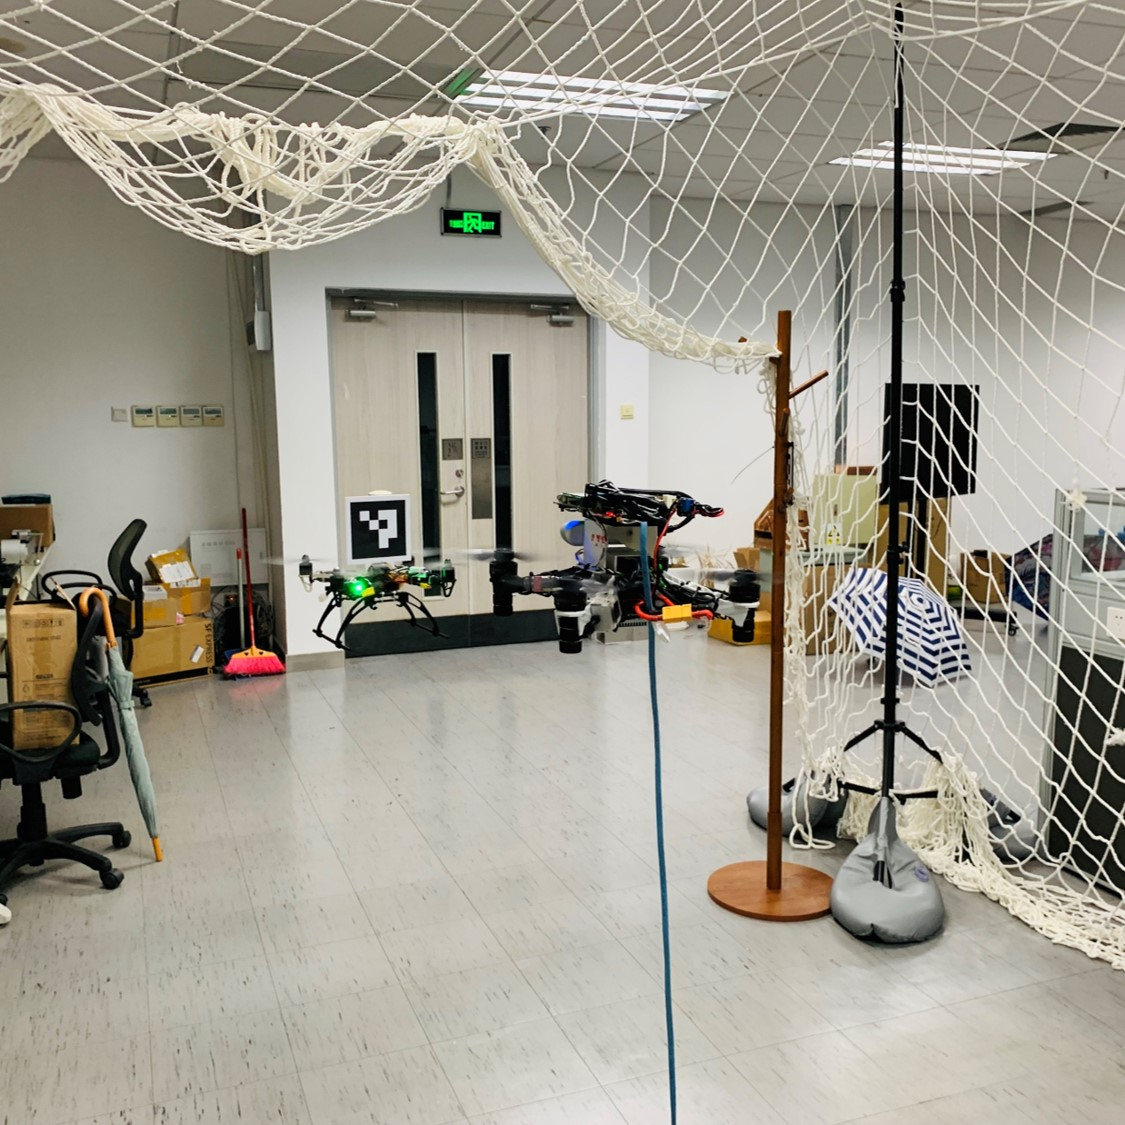
\includegraphics[width=0.49\textwidth]{figure/chapter_1/indoor.jpg}}
  \subfigure[Outdoor environment.]{\label{fig:outdoor}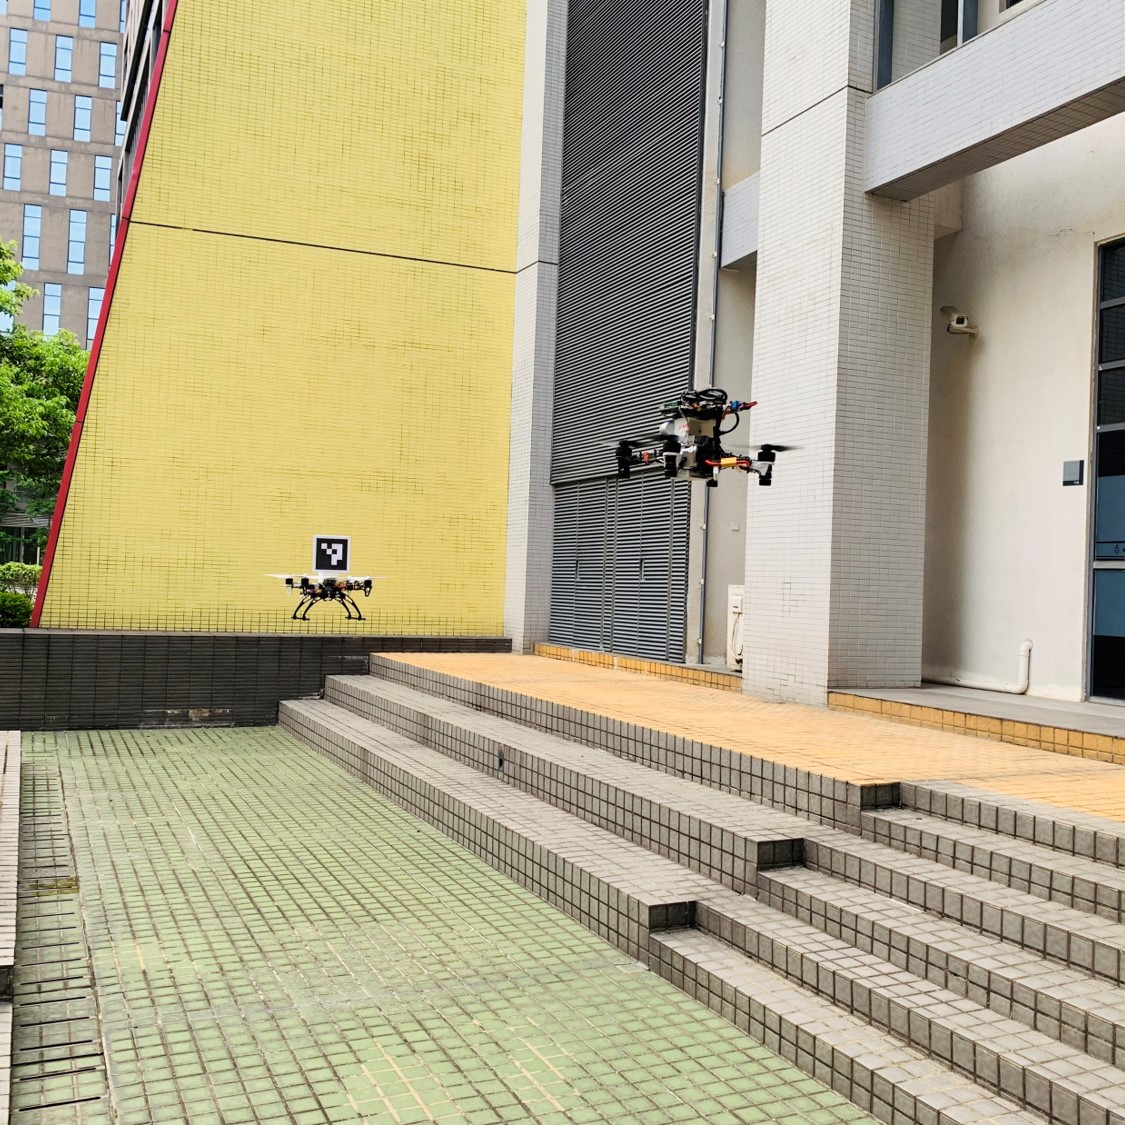
\includegraphics[width=0.49\textwidth]{figure/chapter_1/outdoor.jpg}}
  \caption{Flocking of two UAVs in GPS-denied environments.}\label{fig:indoor_outdoor}
\end{figure}

In this thesis, we present a complete system-level solution to address the aforementioned challenges. The theoretical contribution is the proposal and the proof of a control law satisfying three flocking criteria. The application-level contribution is the design, control and the implementation of the control law using two quadrotors, with the front one being controlled manually and the latter one being fully autonomous as shown in Fig.\ref{fig:indoor_outdoor} and Fig.\ref{fig:twin}. We use the camera as our only on-board sensor for both state estimation and target recognition to maximally imitate natural birds. The flight tests are conducted in both indoor and outdoor environments, and it is successfully demonstrated that our autonomous quadrotor is able to stay flocking with proposed solution.

\begin{figure}[htb]
  \centering
  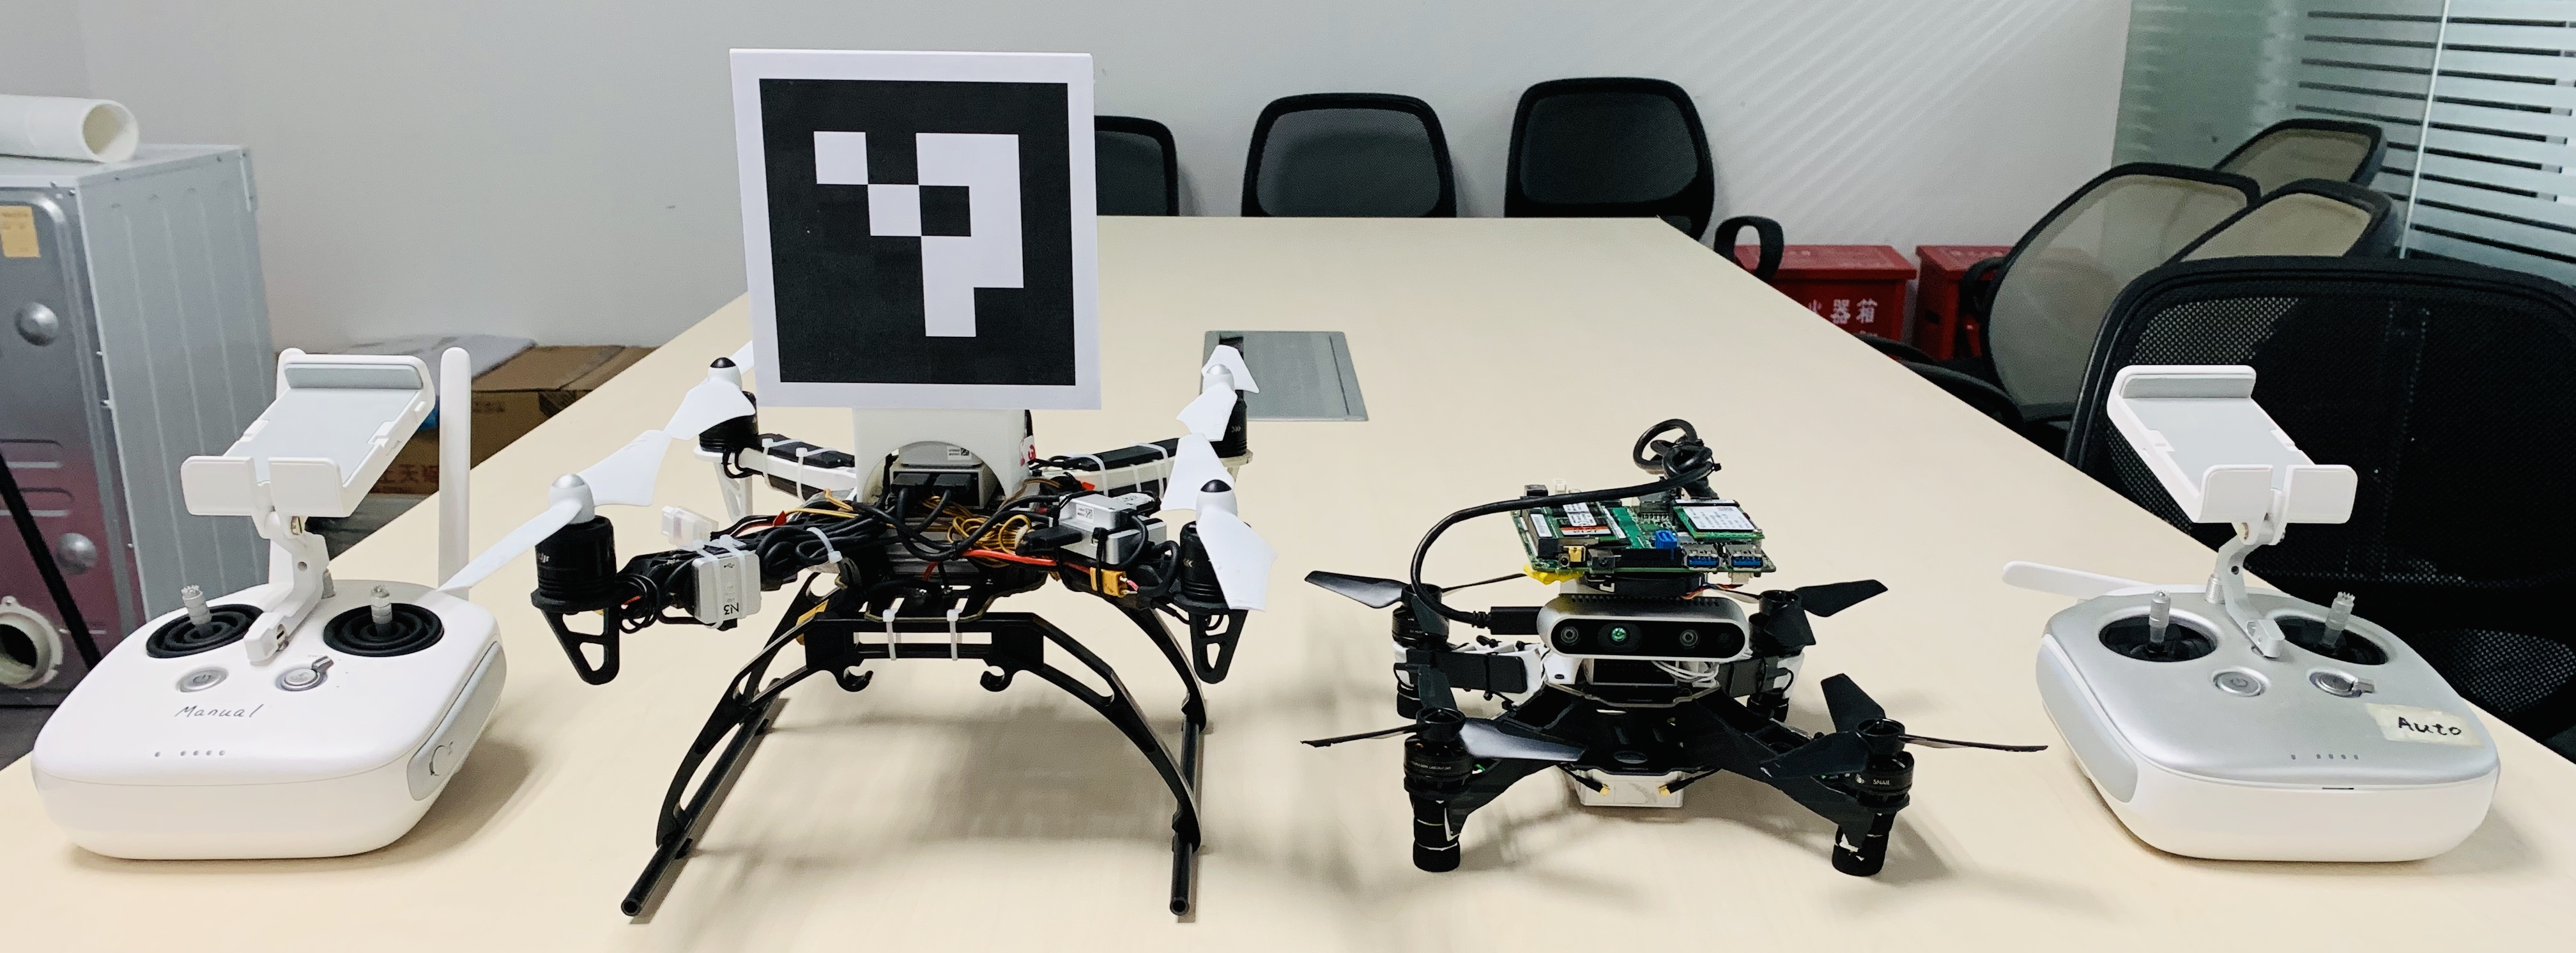
\includegraphics[width=1\textwidth]{figure/chapter_1/all.jpg}
  \caption{Two UAVs where the left one (leader) is manually controlled and the right one (follower) is fully autonomous.}
  \label{fig:twin}
\end{figure}

The outline of the thesis is as follows, Ch.\ref{preliminaries} reviews related theoretical and practical flocking models. Our proposed mathematical model and its proof are shown in Ch.\ref{design}. Ch.\ref{implementation} discusses the architecture and the implementation of our hardware and software platforms. Simulation and real world experiments are shown and in Ch.\ref{experiment}. Ch.\ref{conclusion} concludes this work and points out our possible improvements and future plans.

\newpage
